%\title{Project Report}
%
%%% Preamble
\documentclass[paper=a4, fontsize=11pt]{scrartcl}
\usepackage[T1]{fontenc}
\usepackage{fourier}
\usepackage{listings}

\usepackage[english]{babel}															% English language/hyphenation
\usepackage[protrusion=true,expansion=true]{microtype}	
\usepackage{amsmath,amsfonts,amsthm} % Math packages
\usepackage[pdftex]{graphicx}	
\usepackage{url}
\usepackage{hyperref}
\usepackage{graphicx}
\usepackage{wrapfig}
\usepackage[margin=1.00in]{geometry}
\usepackage{amsmath}

%%% Custom sectioning
\usepackage{sectsty}
\allsectionsfont{\centering \normalfont\scshape}


%%% Custom headers/footers (fancyhdr package)
\usepackage{fancyhdr}
\pagestyle{fancyplain}
\fancyhead{}											% No page header
\fancyfoot[L]{}											% Empty 
\fancyfoot[C]{}											% Empty
\fancyfoot[R]{\thepage}									% Pagenumbering
\renewcommand{\headrulewidth}{0pt}			% Remove header underlines
\renewcommand{\footrulewidth}{0pt}				% Remove footer underlines
\setlength{\headheight}{3.6pt}
\date{}


%%% Equation and float numbering
\numberwithin{equation}{section}		% Equationnumbering: section.eq#
\numberwithin{figure}{section}			% Figurenumbering: section.fig#
\numberwithin{table}{section}				% Tablenumbering: section.tab#


%%% Maketitle metadata
\newcommand{\horrule}[1]{\rule{\linewidth}{#1}} 	% Horizontal rule

\title{
		\vspace{-1in} 	
		\usefont{OT1}{bch}{b}{n}
		\normalfont \normalsize \textsc{Durham Computer Science} \\ [5pt]
		\horrule{0.5pt} \\[0.4cm]
		\large  GPU, Many-core and Cluster Computing Assignment - LLLL76\\
		\horrule{2pt} \\[0.5cm]
		\vspace{-1in} 	
}

%%% Begin document
\begin{document}
\maketitle
\section*{Set Up}

No password on user: user.

%%%%%%%%%%%%%%%%%%%%%%%%%%%%%%%%%%%%%%%%%%%%%%%%%%
\section*{SQL Injection}
\subsection*{Identification}

SQL injection is a technique where SQL commands can be injected into an SQL statement, usually via web page input. In our example, this is possible through the shop that is shown at http://localhost/ in the web browser based on the files found in /var/www/html/.

\subsection*{Exploitation}

This vulnerability can be exploited through the web browser. If both the user name and password fields are set to " ' or 1-1 -- ". This is due to the input not being validated and being used 'as is' in the SQL query that the page does to the database it takes its data from. The query is changed to grant access to the first user in the database, in a slightly more advanced setting the top user is usually the administrator account. In this case the top user has 1000 credits.

\begin{figure}[h]
\centering
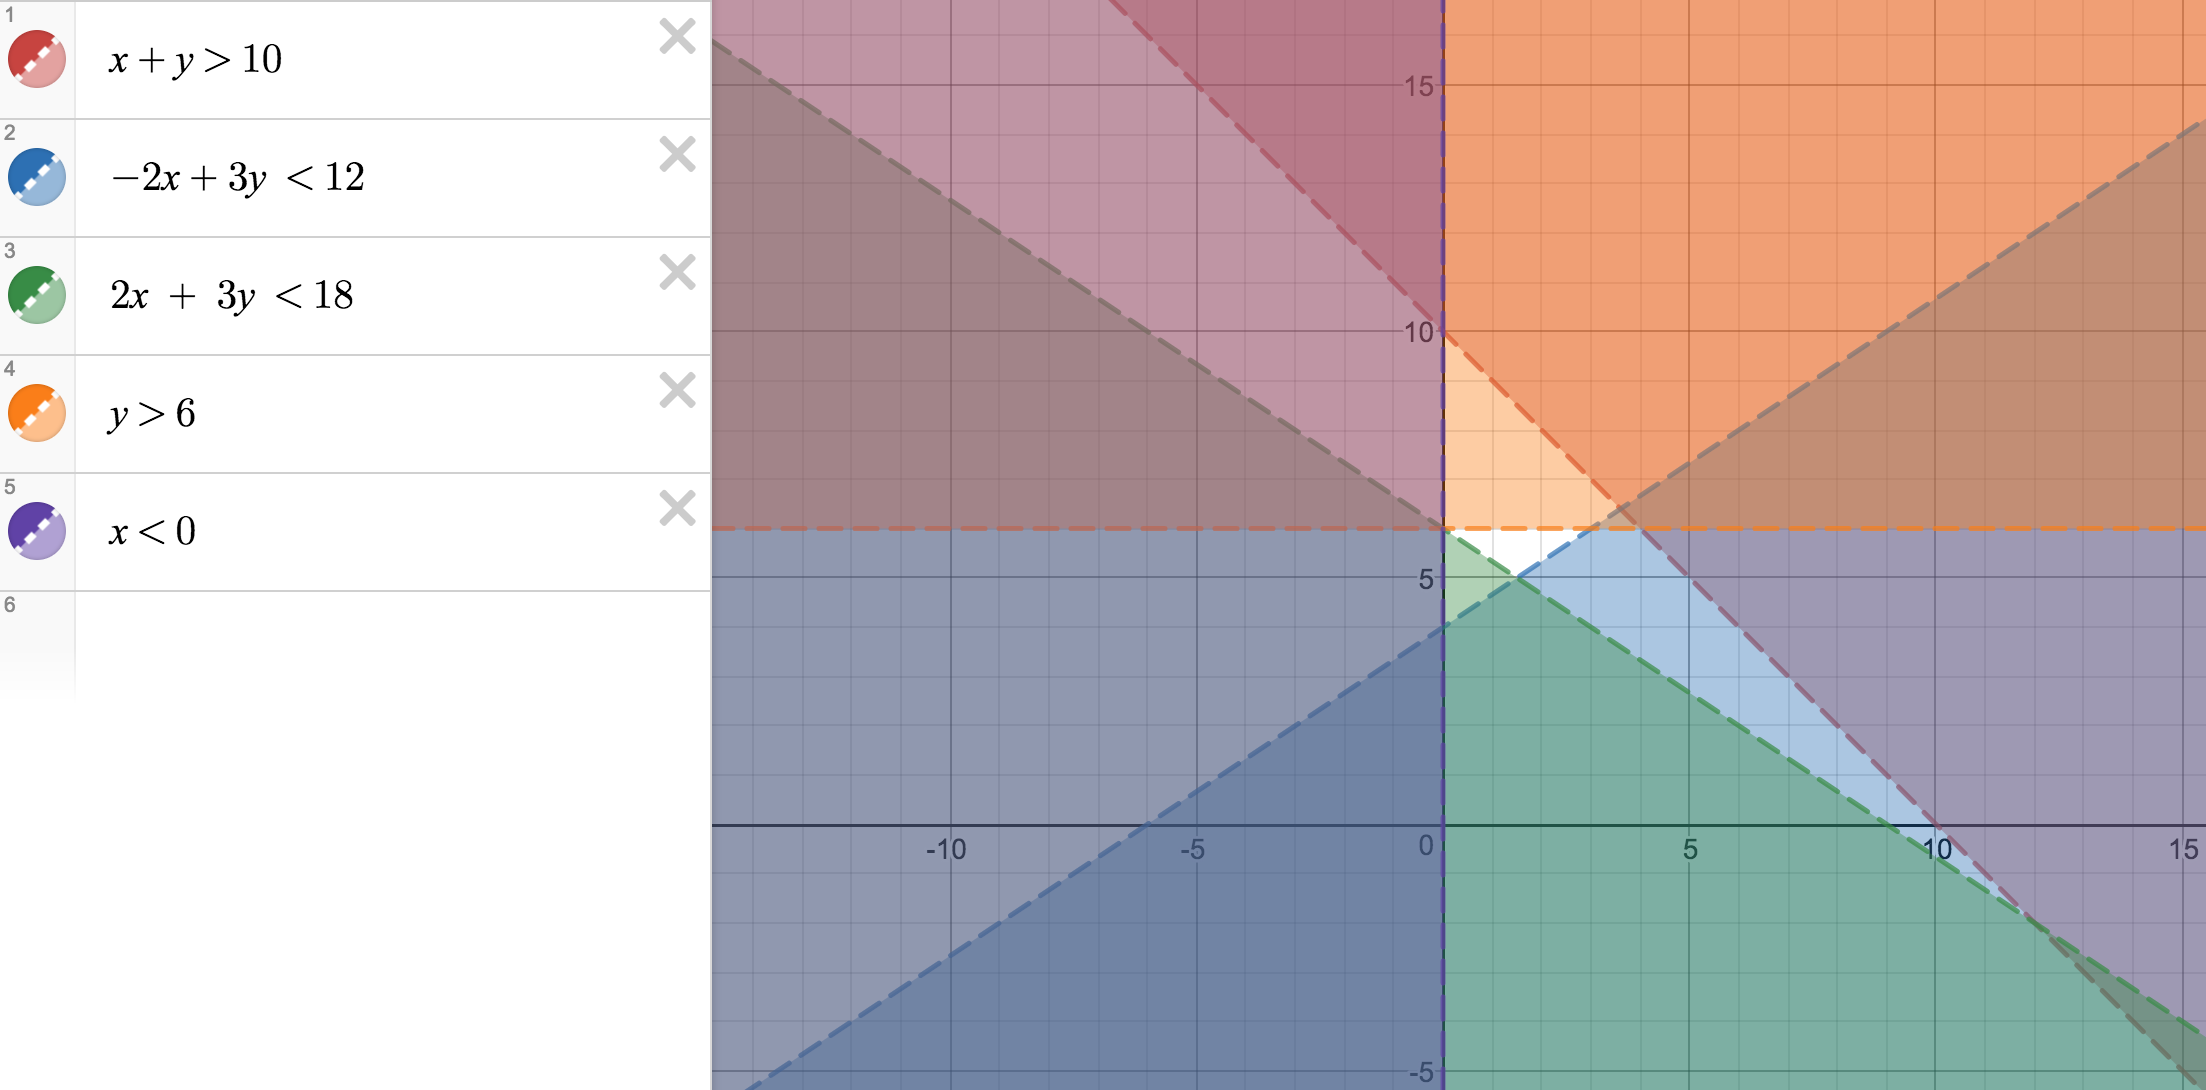
\includegraphics[width=0.75\textwidth]{Pictures/one_one.png}
\end{figure}

\begin{figure}[h]
\centering
\includegraphics[width=0.75\textwidth]{Pictures/one_two.png}
\end{figure}

If we know any of the user names in the database then we can use the same technique to log into any of the accounts and then be able to spend their credits. There are many commands that can be used to exploit this issue, these include changing the number of credits that each user has. Another possibility is getting the passwords file from the 'server' that the SQL is running on.

\subsection*{Mitigation}

The most common way that SQL injection is mitigated is through prepared statements, these are template SQL queries that cannot be changed by any input, as the input are stored as variables and thus are interpreted as separate strings not as part of the SQL query that will be run on the database. An example of a prepared statement is shown below.

Another possibility is a black list. A black list is a list of banned commands that cannot be run on the database, this is not widely used as it can limit the actual functionality of the database.

%%%%%%%%%%%%%%%%%%%%%%%%%%%%%%%%%%%%%%%%%%%%%%%%%%
\section*{Plaintext Passwords}
\subsection*{Identification}

%- where they were found
%- strings command to find them
%- In /var/www/html/
%- Not root read write only they can be accessed from user
%- allows access to the MySQL system with root permissions
%- also used as the root password which makes it much worst

There are passwords stored in plaintext in the directory /var/www/html/. The file that contains the plaintext has permissions such that it can be read from the user account, access of which was given as vulnerability zero. If the source code was not directly available to the user account it could easily be found from the compiled file using the strings command. 

\subsection*{Exploitation}

%- used to change anything in the MySQL database
%- also used to gain root access which can then be used to change almost anything in the system

The password gives access to the MySQL database meaning that anything can be changed in the database, from number of credits to user accounts and passwords to prices of items. This would cause pandemonium to the shop. What makes this vulnerability worse is the fact that the same password is used as the root password. Any malicious individual that had gained access to this file will certainly try the password in as many other situations as possible including using it to try to gain root access. Once root access has been attained the attacker has full access to the system and can change anything at will.

\subsection*{Mitigation}

%- Should not be stored in plaintext
%- Stored in a config file
%- Stored elsewhere on the system thus not accessable if PHP code is leaked from web folder
%- stored hashed
%- stored with the correct permissions

To minimise the damage that this vulnerability can cause the password should be stored in a hashed form, outside of the web directory, which would be accessible to almost anyone. It should also be stored in a config file with root permissions as this would give much more limited access to the more secure hashed password. A final stage of security would be to have different passwords for different parts of the system, meaning that the root password should not be the same as the password for MySQL.

%%%%%%%%%%%%%%%%%%%%%%%%%%%%%%%%%%%%%%%%%%%%%%%%%%
\section*{Permissions}
\subsection*{Identification}

%- .bashrc file has bad permissions
%- all accounts have read and write access

The .bashrc file that can be found in /root/ directory has inappropriate read and write permissions, this file is run every time that bash is called, this includes login. The malicious user being able to edit this file and add or edit bash commands is a significant issue.

\subsection*{Exploitation}

%- what could be done with the file given above

By adding commands such as 'rm -rf *' the 'attacker' could remove all files from the system. The 'attacker' could set all user accounts to root. This file is then run the next time the root user logs in or uses bash and whatever alterations that have been made by the 'attacker' are run.

\subsection*{Mitigation}

%- change the permissions to allow only root access
%- chmod 700 will change to read write and execute permissions to root only

The file should have its permissions changed such that only root can access or change what is in the file. This would mean that only root would be able to change any command that was run from the .bashrc file. The permissions would be changed by running the command chmod, in this case chmod 700 .bashrc, this command should be used in many other cases throughout the system but this is the most significant flaw that could be found and so will be directly addressed whilst other permission issues will just be mentioned in passing. 

%%%%%%%%%%%%%%%%%%%%%%%%%%%%%%%%%%%%%%%%%%%%%%%%%%
\section*{Command Injection}
\subsection*{Identification}

%- use a file with elevated permissions to allow the 'attacker' to run commands they would otherwise not be able to run
%- this is possible in outputDB file

The outputDB file is vulnerable to command injection. The source code can be read by any user and we can see from reading the source that the line ' setuid(0) ' is used to allow the running of privileged commands. This allows the 'attacker' to run commands that they otherwise would not be able to.

\subsection*{Exploitation}

%- a root shell can be accessed
%- allowing full control of the system

To allow for access to a root terminal the command ' ./outputDB " database.txt \&\& bash " ' is run after the non root user navigates to the home directory. This works because the input to the code is simply appended to the end of a predefined command and not validated in any way.

\subsection*{Mitigation}

%- shouldn't pass user information to system() function
%- use execve() instead
%- this will only ever run the hardcoded commands

We can see in the code that the command line arguments are concatenated with the hardcoded command in the code and then run using the system() command. The system() command should not be used in this case, instead the command execve() should be used instead of the concatenation and system commands. An example of the execve() command in use: ' execve(cmd, args) '. The system command is insecure and will run any command it is passed where as the execve() command will treat any arguments after \&\& or similar symbols as text arguments and not as part of the command that should be run.

%%%%%%%%%%%%%%%%%%%%%%%%%%%%%%%%%%%%%%%%%%%%%%%%%%
\section*{Weak Passwords}
\subsection*{Identification}

%- the system does not have a passwd shadow file and thus stores the hashed passwords and their corresponding salt in the /etc/passwd file. They are very weak passwords such as 'letmein'

The system does not have a passwd shadow file, this file would be used to store passwords in their hashed form along with the salt used in the hashing in a root readable file separate from all other information. Due to the lack of this file the passwords in their hashed form with corresponding salt are stored in the /etc/passwd/ file that is universally accessible.

\subsection*{Exploitation}

%- once the file has been found
%- can be cracked using John the Ripper

If the passwd file is found and the hashed passwords are known to a malicious user then it is only a matter of time before these passwords are broken. There are many tools available to break such passwords, a dictionary attack would be the most common with specialised tools such as 'John-The-Ripper' being utilised to find the passwords fairly quickly. The time taken for the dictionary attack to work is significantly reduced by the strength of the passwords that the system uses, ' letmein, 1234567, and password '.

\subsection*{Mitigation}

%- system should use a correctly configured shadow file 
%- this will store the passwords in a similar fashion but they are only accessible from root

Set up a working shadow file to store the passwords, making sure that all the permissions are correct, root accessible only. Also changing the hashing function used from MD5 to something more secure as MD5 has been shown to have extensive vulnerabilities. Using a hashing algorithm with a higher security claim such as SHA256 would be better got the security of the system.

%%%%%%%%%%%%%%%%%%%%%%%%%%%%%%%%%%%%%%%%%%%%%%%%%%
\section*{Cross-Site Scripting}
\subsection*{Identification}

%- Cross-Site Scripting what it is
%- how it would be done to the database

Cross-Site Scripting is a vulnerability typically found in web applications. XXS enables client side scripts to be injected into the web pages so as to cause damage. In this instance it is possible either through the mysql framework or via SQL injection into the shop homepage. 

\subsection*{Exploitation}

%- from SQL injection or from direct access to the mySQL shell
%- how the database must be changed to allow for a script to be run
%- show that a script can be run

Using the MySQL shell we can alter a column in the database to allow for commands to be input instead of the data that it expects. In this case it would be fairly simple to change the credits column to accept varcharr(300) instead of the integer it is expecting. Once this has been done then any command can be input into the column, an example of this would be some HTML code that would cause multiple alerts to trigger when the webpage was loaded. Any command input into the database is usually surrounded by <script> tags.

\subsection*{Mitigation}

%- white list of commands that can be run by privileged users

To limit the possibility of this the database should have more limitations on who can access and make changes to it and the web page should have more security against SQL injection. An extreme solution would be to make the SQL tables immutable such that the formats of the tables cannot be changed to allow for anything other than what they were specifically designed for to be input into each column, this has the drawback of limiting the functionality of the database. A less extreme option is to limit the commands that can be run on the database and also limit the users that are allowed to perform them, for example to change the structure of the table, the user must have higher permissions than a standard user, where as to query and add data this can be done from a standard user who knows the basic MySQL password.

%%%%%%%%%%%%%%%%%%%%%%%%%%%%%%%%%%%%%%%%%%%%%%%%%%
\section*{Database Misconfiguration}
\subsection*{Identification}

%- all users can use the database
%- all passwords in the database are shown in plaintext 

There is not limitation on user access to the MySQL database.

\subsection*{Exploitation}

%- show list of commands to gain access to passwords
%- all the passwords are changeable, all the prices are changeable
%- havoc for the shop

Open a terminal as any user and type mysql, this will give access to the full, unencrypted database. This will allow any user to change anything in the tables. This includes changing passwords, adding users with very large amounts of credits, changing prices for things in the shop and being able to read the passwords of other users that are stored in plaintext.

\subsection*{Mitigation}

%- reconfigure mysql with root permissions
%	- remove all other users
%	- add a password for the root user
%	- restart SQL
%- make sure only root has access to users table
%- limit queries that can be done on the database by non root users
%- store all passwords in hashed form

The first step to reconfigure the database would be to remove all access that was not root on the system. This would be simple enough to do using the DELETE command to remove all other users of the database. The next step would be to create additional security measures by adding a MySQL specific password to the database. The final stage would be to limit access to the plaintext passwords of other users, this would be done by creating another level of privilege in MySQL, such that only users that have this higher permission could access the users table. To further cement this the passwords should not be stored in plaintext they should be hashed using an up to date hashing algorithm such as SHA256. Further measures include limiting queries of lower privileged users and limiting the commands that they can run on the database.

%%%%%%%%%%%%%%%%%%%%%%%%%%%%%%%%%%%%%%%%%%%%%%%%%%
\section*{TOCTTOU}
\subsection*{Identification}

%- Time Of Creation To Time Of Use
%- The hourly backup of the database in readable by the user before it is deleted

A time of check to time of use attack is a vulnerability caused by the delay on a system between the time of a checking of a condition and the time of the use of that result. In this case the time taken between the hourly backup script creating a file that contains the backup database and the time taking to send and delete the file. 

\subsection*{Exploitation}

%- a small script could be created to take a copy of this database before it is deleted locally
%- the whole database is then readable by the 'attacker'

This vulerability would be easily exploited by a small script that constanly checks for the presence of the file and at the time it is created make a clone with a different name and either send it to another directory to be sent on at a later date or just broadcast it across the network. This vulnerability is made worse by the permissions the backup file has, it is completely open and is readable by any user.

\subsection*{Mitigation}

%- store the database in memory
%- issue for large databases that may be bigger than memory
%- if this is the case then it can be output as a file as long as it is encrypted
%- this may cause a bit of overhead

A possibility is to store the database in system memory and not create the file but this has similar issues to just creating the file, we have simply moved the problem to somewhere else, we also have the added issue of possibly running out of system memory for a larger database. The best way would be through encryption and strict permissions, the database can be created in the current directory as long as the permissions are such that only another new user account can access the relevant files, and even if they were accessible by another user then they are encrypted which whilst not being unbreakable is better than having them in plaintext. This solution is not perfect and could be broken given time and patience but is much better than the current set up.

%%%%%%%%%%%%%%%%%%%%%%%%%%%%%%%%%%%%%%%%%%%%%%%%%%
%%% End document
\end{document}